% !TeX spellcheck = en_US
\documentclass{article}
\usepackage{graphicx}
\usepackage{fancybox}
\usepackage{tikz}
\usepackage{algorithm}
\usepackage{amsmath}
\usepackage{algorithmicx}
\usepackage{hyperref}
\usepackage{algpseudocode}
\usepackage{graphicx}
\usepackage{caption}

\captionsetup{labelfont={color=black,bf}}

\makeatletter
\def\BState{\State\hskip-\ALG@thistlm}
\makeatother

\algdef{SE}[DOWHILE]{Do}{doWhile}{\algorithmicdo}[1]{\algorithmicwhile\ #1}%

\title{Homework 01: Matrix Multiplication}
\date{\today}
\author{Roberto Corti}

\begin{document}
	\maketitle
	
	
	\noindent \textbf{Clone the Strassen’s project template from}. 
	\begin{center}
		\url{https://github.com/albertocasagrande/AD_strassen_template} 	
	\end{center}
	\textbf{and solve the following exercises.}
	
	
	\section*{Exercise 1}
	\textbf{Generalize the implementation to deal with non-square matrices.}\\
	
	\noindent The implementation is written in the file \texttt{src/rectangular.c} by the function \texttt{strassen\_rectangular} \texttt{\_multiplication}.
	\\
	
	\noindent In order to deal with rectangular matrices, the idea of this implementation is to embed squared matrices whose size is not a power of two into squared matrices having size equal to the smaller power of two bigger than the original size through a \textit{padding} operation.\\
	Once having this generalization to square matrices, if the input matrices are rectangular they are then divided to square blocks having size a power of two. Given this operation, the rectangular matrix multiplication will be given by a block-wise Strassen's multiplication followed by a sum of the partial results.
	
	\section*{Exercise 2}
	\textbf{Improve the implementation of the Strassen’s algorithm by reducing the memory allocations and test the effects on the execution time.}\\
	
	\noindent The implementation is written in the file \texttt{src/strassen.c} by the function \texttt{strassen\_matrix\_multiplication\_opt}.
	\\
	
	\noindent In order to have a more efficient use of memory, instead of allocating 17 matrices (10 for $S$, 7 for $P$) as the original code of Strassen does, I decided to allocate only 6 of these (2 for $S$ and 4 for $P$) and use a sequential calculation that updates multiple times the value of these matrices in order to compute the blocks $C_{11}, C_{12}, C_{21}, C_{22}$. \\
	Once written this optimized version, I performed a test with the original implementation and the results are shown by the graph in Figure 1.

	\begin{figure}[h]
		\begin{center}
			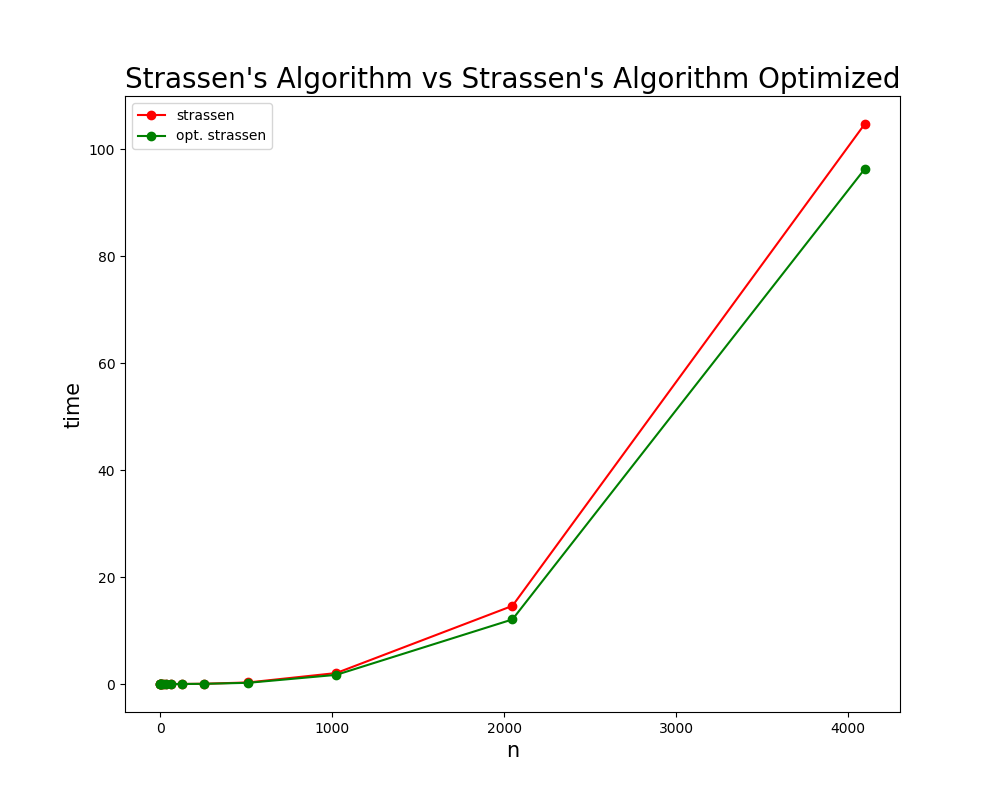
\includegraphics[width=.8\textwidth]{../data/plot.png}
			\label{plot}
			\caption{Time performance of the two implementations of the Strassen's Algorithm}
		\end{center}
	\end{figure}	
	
	
\end{document}